\begin{figure*}[t]
    \centering

    \begin{subfigure}[t]{0.32\linewidth}
        \centering
        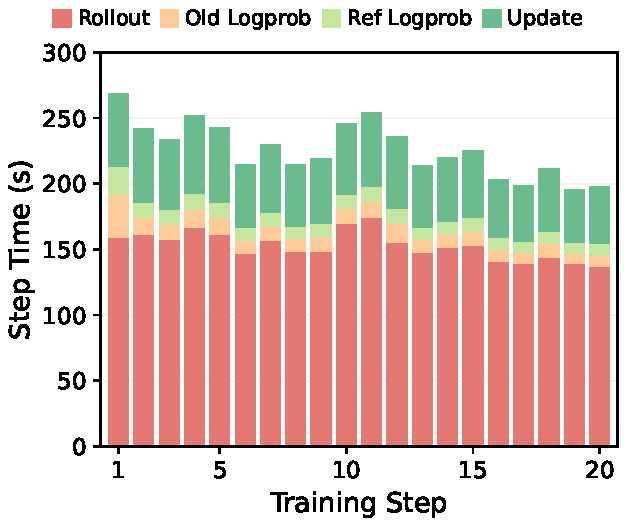
\includegraphics[width=\linewidth]{figures/main_rollout_step_time_llama8b.pdf}
        \caption{}
        \label{fig:rollout_llama_bottleneck_step}
    \end{subfigure}
    \hfill
    \begin{subfigure}[t]{0.32\linewidth}
        \centering
        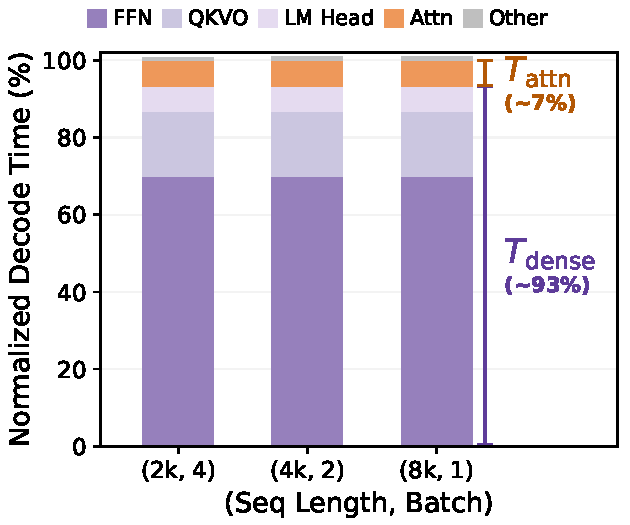
\includegraphics[width=\linewidth]{figures/main_rollout_decode_breakdown_llama_8b.pdf}
        \caption{}
        \label{fig:rollout_llama_decode_breakdown}
    \end{subfigure}
    \hfill
    \begin{subfigure}[t]{0.32\linewidth}
        \centering
        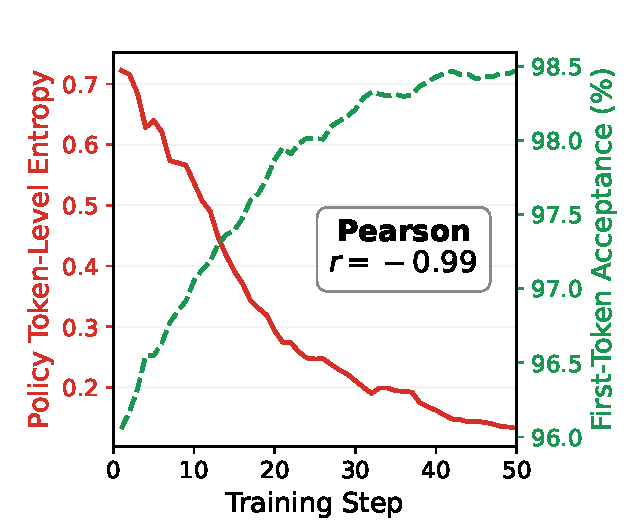
\includegraphics[width=\linewidth]{figures/main_motivation_entropy_acc_qwen7b.pdf}
        \caption{}
        \label{fig:entropy_acceptance_qwen}
    \end{subfigure}

    \caption{
    \textbf{Empirical characteristics of RL rollout decoding.}
    (a) Step-time decomposition over the first 20 training steps.
    (b) Single-token decode-time breakdown in RL rollout-tail phases.
    (c) Inverse correlation between target-policy entropy and quantized-drafter first-token acceptance over steps.
    }
    \label{fig:rollout_bottleneck}
\end{figure*}

\section{{\methodtitle{}: From RL Rollout Dynamics to System-Aware Self-SD}}
\label{sec:method}

This section develops \textbf{\methodtitle{}} from three RL rollout characteristics.
First, the evolving target policy and rollout-tail latency profile motivate a weight-quantized drafter for self-SD.
Second, shifting runtime regimes motivate an SD toggle policy that activates only when beneficial.
Third, changing acceptance behavior during RL motivates adaptive draft lengths.
We describe each component below; \Cref{alg:full-pipeline} summarizes the full \methodtitle{} pipeline for~\cref{subsec:target-induced-drafter,subsec:sd-toggle,subsec:adaptive-gamma}.

\subsection{Weight-Quantized Drafter for Self-Speculative Decoding}
\label{subsec:target-induced-drafter}

\textbf{Self-speculative decoding.}
Among the SD designs in \cref{tab:rl_sd_taxonomy}, self-SD with a target-induced drafter~\citep{zhang2024draft,yue2026specattn,tiwari2025quantspec} is well suited to RL, where the target model evolves throughout training.
Because the drafter is derived directly from the current target, it remains synchronized with the evolving policy without separate drafter pretraining or online adaptation.
This contrasts with learned auxiliary drafters, which can become stale unless continually adapted online to track the evolving policy~\citep{zhang2025fastgrpo}.


\textbf{Rollout-tail latency decomposition.}
We decompose rollout-tail single-token decoding latency, $\Tdecode$, to identify which component a self-SD drafter should make cheaper.
As shown in \cref{fig:rollout_llama_decode_breakdown}, dense projection time $\Tdense$, including QKVO, FFN, and LM-head projections, accounts for around 90\% of total latency, exceeding attention time $\Tattn$ by more than $10\times$.
This observation is consistent with modern LLM architectures that reduce KV-cache sizes~\citep{shazeer2019fast,ainslie2023gqa,liu2024deepseek,guo2025deepseek} and with system analyses showing that parameter loading dominates latency in small-batch memory-bound regimes~\citep{sadhukhan2024magicdec}.

\textbf{Weight-quantized drafting.}
We induce a weight-quantized drafter~\citep{tiwari2025quantspec} from the current target model to reduce the weight-loading cost of $\Tdense$, the dominant component of rollout-tail latency (\cref{fig:rollout_llama_decode_breakdown}).
This lowers the drafter-to-target latency ratio $\DraftTime/\TargetTime$ in~\cref{eq:sd_speedup}.
Specifically, we apply lightweight RTN quantization to the FFN and QKVO projection layers at the beginning of each training step, following prior practice~\citep{lin2024awq}.
We use 4-bit weights (W4) as a practical latency--acceptance trade-off: lower precision makes drafting substantially cheaper while preserving sufficient block efficiency $\mal$ for effective SD.
In contrast, sparse-attention drafting, another representative self-SD approach, mainly targets $\Tattn$, which contributes far less than $\Tdense$ to rollout-tail latency in this regime.
Layer skipping is also a self-SD option; however, fixed skipping patterns often provide limited practical speedup~\citep{xia2024unlocking,song2026knn}, while adaptive skipping is difficult to combine with static inference optimizations in modern serving engines, such as CUDA graph pre-capture~\citep{xia2024swift,chen2025clasp,kwon2023efficient}.
\Cref{app:w4_vs_w8,app:practical_quantized_vs_sparse} further analyze self-SD alternatives and W4--W8 latency--acceptance trade-off.


\subsection{Regime-Aware SD Toggle Policy via Roofline Modeling}
\label{subsec:sd-toggle}

Even with a cheap quantized drafter, SD is not beneficial throughout the entire rollout.
Early rollout phases have large active batches that can saturate compute, leaving little underutilized compute for target verification (\ie{}high $\VerifyTime/\TargetTime$ in~\cref{eq:sd_speedup}). As a result, SD can be slower than AR decoding despite high $\mal$.
As shorter responses finish, the active batch shrinks and decoding enters a low-batch tail where SD becomes beneficial.
To decide when to enable SD, we use a roofline model to predict speedup (\cref{subsec:roofline-latency}) from the current decoding state $(B,S)$ and SD runtime state $(\mal,\gamma)$, activating SD only when the prediction is favorable.

\textbf{SD toggle policy.} 
To implement this decision, the SD toggle policy uses a calibrated model to predict the SD-over-AR speedup for the current decoding state $(B,S)$.
We first define memory-side and compute-side cost estimates for target, draft, and verification execution:
\begin{equation*}
\TargetMemory
=
\frac{\TargetWeights+\KVTrafficCoeff BS}{\EffBandwidth},
\quad
\DrafterMemory
=
\frac{\DrafterQuantCoeff\DrafterWeights+\KVTrafficCoeff BS}{\EffBandwidth},
\quad
\ForwardCompute
=
\frac{B(\DenseCompute+S\AttnCompute)}{\mathrm{F}_{\mathrm{eff}}}.
\end{equation*}
Here, $\TargetMemory$ and $\DrafterMemory$ estimate data-movement costs for one target or quantized-drafter forward pass, including weight and effective KV-cache traffic, while $\ForwardCompute$ estimates the arithmetic cost of one forward pass.
$\TargetWeights$ and $\DrafterWeights$ denote the target and drafter weight sizes, respectively, and $\DenseCompute$ and $\AttnCompute$ denote architecture-determined dense and attention compute costs.
Because the target and self-drafter share the same architecture, they share the same compute term; the quantized drafter's reduced weight traffic is captured by $\DrafterQuantCoeff$ in the memory-side term.
Using~\cref{eq:roofline_basic}, we instantiate the roofline latency for target decoding, quantized-drafter decoding, and target verification as
\begin{equation*}
\widehat{\TargetTime}
=
\max\{\TargetMemory,\ForwardCompute\}
+
\TargetOverhead B,
\quad
\widehat{\DraftTime}
=
\max\{\DrafterMemory,\ForwardCompute\}
+
\DrafterOverhead B,
\quad
\widehat{\VerifyTime}
=
\max\{\TargetMemory,(\DraftLength+1)\ForwardCompute\}
+
\VerifyOverhead B.
\label{eq:toggle_latencies}
\end{equation*}
The overhead terms capture non-ideal overlap and batch-dependent residual costs beyond ideal roofline approximation.
Following the SD speedup model in~\cref{eq:sd_speedup}, we define the SD toggle policy $\SDToggle$ to activate SD when the predicted speedup exceeds a safety margin:
\begin{equation}
\SDToggle(B,S,\mal,\DraftLength)
=
\mathbf{1}
\left[
\frac{
\mal\,\widehat{\TargetTime}
}{
\DraftLength\widehat{\DraftTime}
+
\widehat{\VerifyTime}
}
\geq
1+\ToggleMargin
\right],
\qquad
\ToggleMargin\geq0.
\label{eq:sd_speedup_toggle}
\end{equation}
Once activated, SD remains enabled until the end of the rollout, as the active batch size monotonically decreases toward the SD-beneficial tail regimes.

\textbf{Calibrated parameters.}
We introduce additional calibration parameters to adapt the roofline model and the corresponding policy to different model and system configurations.
The fitted terms $\KVTrafficCoeff$, $\DrafterQuantCoeff$, and 
$\TargetOverhead,\DrafterOverhead,\VerifyOverhead$ capture effective KV-cache traffic, quantized-drafter effects, and residual per-batch overheads for target, draft, and verification execution, respectively.
These parameters are calibrated once per model--hardware pair using a pre-hoc profiling sweep and can be reused across RL runs. \Cref{app:toggle_calibration} provides calibration details.


\subsection{Adaptive Draft-Length Policy}
\label{subsec:adaptive-gamma}

\paragraph{Acceptance behavior evolves during RL.}
The weight-quantized drafter can become more effective over training, increasing $\tau$ as RL sharpens the target policy.
In \cref{fig:entropy_acceptance_qwen}, target-output entropy and token-level agreement between $\Target$ and its weight-quantized copy $\TargetQuantized$ show a strong negative correlation ($r=-0.99$).
As training progresses, RL can reduce target-output entropy~\citep{jin2025revisiting,cui2025entropy}, sharpening the target policy by concentrating probability mass on a smaller set of high-reward tokens~\citep{huang2024self,yang2025llm}.
A sharper distribution can make top-token decisions less sensitive to small quantization-induced perturbations, increasing agreement between $\Target$ and $\TargetQuantized$.
Consistent with this explanation, we observe that the quantized self-drafter's $\tau$ improves over training, motivating adaptive draft budgets that increase as acceptance improves.
\Cref{app:entropy_acceptance} provides full experimental results for policy sharpening and block-efficiency improvement.

\paragraph{Adaptive policy for draft length $\gamma$.}
To exploit the increasing $\tau$ observed during RL training, we choose the next draft length $\gamma_{t+1}$ using the measured block efficiency $\mal_t$ as a proxy for current drafter quality.
We maintain an ordered draft-length set $\Gamma=[\gamma_{\mathrm{low}},\dots,\gamma_{\mathrm{high}}]$ and update from $\gamma_t$ to $\gamma_{t+1}$ only when the condition on $\mal_t$ persists for $P$ consecutive training steps.
Specifically, we increase the draft length when $\mal_t$ is close to the current draft-length ceiling, and decrease it when acceptance is too low to amortize draft computation.
The patience window $P$ prevents transient fluctuations in $\mal_t$ across steps from changing the draft length.
This removes the need to select a single fixed $\DraftLength$ through post-hoc sweeps, instead letting the adaptive policy move within a pre-specified draft-length set using observed $\mal_t$ feedback during RL training.

\begin{algorithm}[t]
\caption{\methodtitle{} Pipeline}
\label{alg:full-pipeline}
{\textbf{Parameter}:} draft-length set $\Gamma=[\gamma_{\mathrm{low}},\dots,\gamma_{\mathrm{high}}]$, toggle margin $\ToggleMargin$, block-efficiency thresholds $\alpha_{\mathrm{up}},\alpha_{\mathrm{down}}$, patience $P$\\
{\textbf{Input}:} target model, rollout states with runtime batch size $B$, and sequence length $S$.
\begin{algorithmic}[1]
\State Initialize $\gamma_1 \gets \gamma_{\mathrm{low}}$ and $\mal_0 \gets \gamma_{\mathrm{low}}$
\For{training timestep $t=1,2,\dots$}
    \State Refresh the drafter by quantizing the current target model
    \State Initialize $\SDOn \gets \textbf{false}$
    \While{rollout not finished}
        \If{$\SDOn=\textbf{false}$ and $\SDToggle(B,S,\mal_{t-1},\gamma_t)=0$}
            \State Decode autoregressively
        \ElsIf{$\SDOn=\textbf{false}$ and $\SDToggle(B,S,\mal_{t-1},\gamma_t)=1$}
            \State $\SDOn \gets \textbf{true}$
        \Else
            \State Decode with SD using draft length $\gamma_t$
        \EndIf
    \EndWhile
    \State Measure step-level block efficiency $\mal_t$
    \State $\gamma_{t+1} \gets
    \begin{cases}
    \mathrm{next}_{\Gamma}(\gamma_t),
    & \min\limits_{t' \in [t-P+1,t]} \mal_{t'} \ge 1+\gamma_t\alpha_{\mathrm{up}},\ \gamma_t<\gamma_{\mathrm{high}}, \\
    \mathrm{prev}_{\Gamma}(\gamma_t),
    & \max\limits_{t' \in [t-P+1,t]} \mal_{t'} \le 1+\gamma_t\alpha_{\mathrm{down}},\ \gamma_t>\gamma_{\mathrm{low}}, \\
    \gamma_t,
    & \text{otherwise.}
    \end{cases}$
    \State Run standard post-rollout optimization
\EndFor
\end{algorithmic}
\end{algorithm}

% \begin{algorithm}[t]
% \caption{\methodtitle{} Runtime Policy}
% \label{alg:full-pipeline}
% {\textbf{Parameter}:} initial draft length $\gamma_0$, draft-length set $\Gamma=[\gamma_{\mathrm{low}},\dots,\gamma_{\mathrm{high}}]$, toggle margin $\epsilon$, block-efficiency thresholds $\alpha_{\mathrm{up}},\alpha_{\mathrm{down}}$, patience $P$\\
% {\textbf{Input}:} target model, rollout states with runtime batch size $B$, and sequence length $S$.
% \begin{algorithmic}[1]
% \State Initialize $\gamma \gets \gamma_0$ and $\mal_{\mathrm{prev}} \gets \gamma_0$
% \For{training timestep $t$}
%     \State Refresh the drafter by quantizing the current target model
%     \State Initialize $\SDOn \gets \textbf{false}$
%     \While{rollout not finished}\mj{express prev using t}
%         \If{$\SDOn=\textbf{false}$ and $\SDToggle(B,S,\mal_{\mathrm{prev}},\gamma)=0$}
%             \State Decode autoregressively
%         \ElsIf{$\SDOn=\textbf{false}$ and $\SDToggle(B,S,\mal_{\mathrm{prev}},\gamma)=1$}
%             \State $\SDOn \gets \textbf{true}$
%         \Else
%             \State Decode with SD using draft length $\gamma$
%         \EndIf
%     \EndWhile
%     \State Measure step-level block efficiency $\mal$
%     \State Update $\gamma \gets
%     \begin{cases}
%     \mathrm{next}_{\Gamma}(\gamma),
%     & \min\limits_{t' \in [t-P+1,t]} \mal_{t'} \ge 1+\gamma\alpha_{\mathrm{up}},\ \gamma<\gamma_{\mathrm{high}}, \\
%     \mathrm{prev}_{\Gamma}(\gamma),
%     & \max\limits_{t' \in [t-P+1,t]} \mal_{t'} \le 1+\gamma\alpha_{\mathrm{down}},\ \gamma>\gamma_{\mathrm{low}}, \\
%     \gamma,
%     & \text{otherwise.}
%     \end{cases}$
%     \State $\mal_{\mathrm{prev}} \gets \mal$
%     \State Run standard post-rollout optimization
% \EndFor
% \end{algorithmic}
% \end{algorithm}


